\chapter*{Doorn}

\lettrine[lines=2, loversize=0.3, lraise=0]{\initfamily J}{oop} kwam een keer thuis van een reis en hij zei: ``We gaan een huis kopen! We kunnen wel blijven sparen, maar we nemen gewoon een hypotheek.'' Dan draag je regelmatig geld af en omdat hij een goeie baan had kon dat best. 

Toen zijn we in Doorn terecht gekomen, want ik dacht: ``Ik ga niet in Schoorl wonen''. Dat leek me niet goed. Zo zaten we centraal, want hij moest soms ook bijwerken en dan moest hij naar Rotterdam, of Amsterdam en dat was te doen.

Het was wel fantastisch natuurlijk om een eigen huis te hebben. Het huis had een ander laten bouwen, maar die ging er uiteindelijk niet in. 

\begin{figure}[h]
    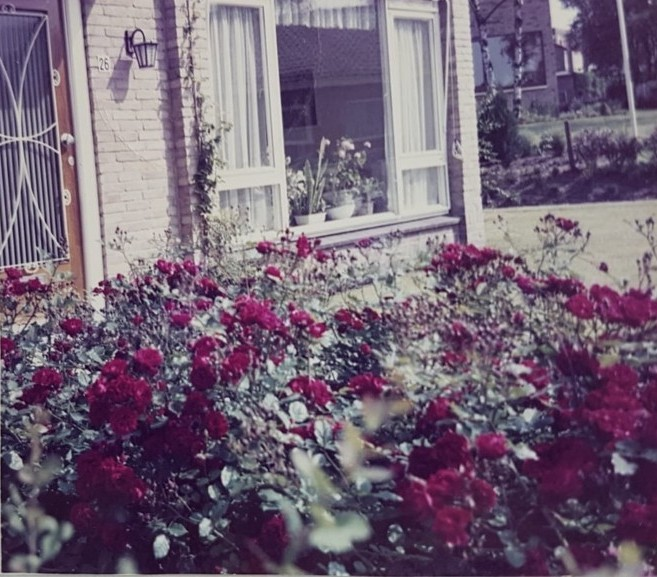
\includegraphics[width=\textwidth]{image50}
    \caption{Het huis in Doorn.}
\end{figure}

Het was fijn aan de rand van het bos. Er hingen ook wel eekhoorntjes aan de pinda’s. Ik was wel blij dat we dat huis hadden, dat we daar gingen wonen. Want een appartement was ik niet gewend natuurlijk. Ik miste een tuin.

Al gauw kwam ‘tante’ Betty er wonen met haar man en ook de familie van Putten. Die gingen eerder al weer weg. Daar zijn we ook nog geweest, op de Veluwe. (dat weet dochter Yvonne nog goed..zij speelde zo graag met Tink).

Tegenover woonde Toek Beekman (tante Toekie) met haar man. Ik kon wel met haar omgaan. Ik moest wel om haar lachen, maar de kapiteins zeiden: ``Ik wil die vrouw niet meer aan boord hebben''. Als pappa de auto ging schoonmaken, was ze er ook ineens. Ze hing om andere mannen heen blijkbaar. Maar ik ben wel steeds gewoon met haar omgegaan.

\begin{figure}[h]
    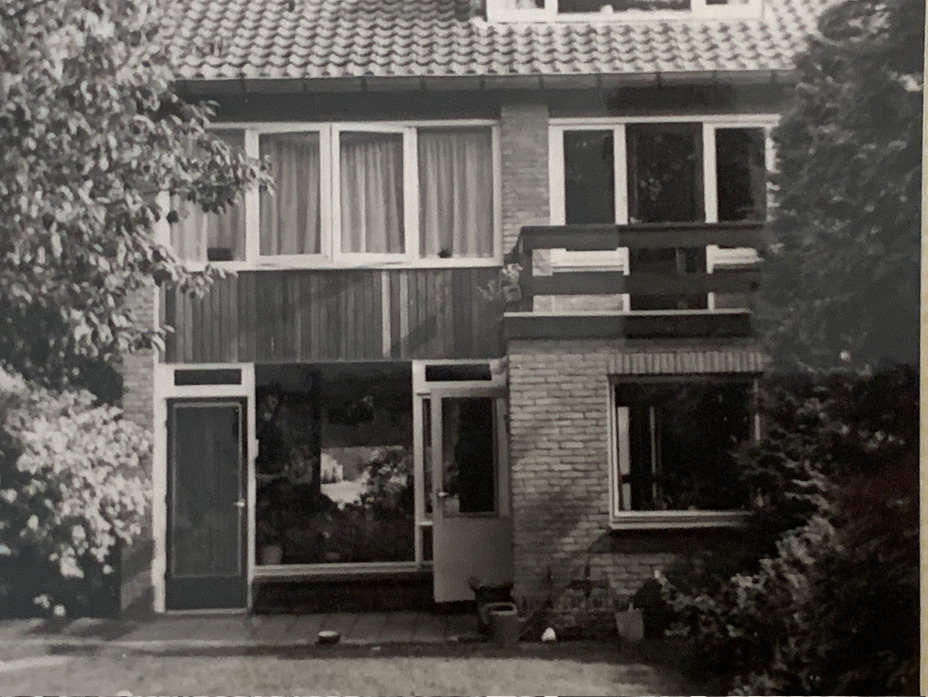
\includegraphics[width=\textwidth]{image51}
    \caption{Ons huis.}
\end{figure}

Ja, we hebben daar altijd wel lekker gewoond, hoor. Om dat pleintje. Ik zie de kinderen nog die bult op fietsen. Eerst bracht ik ze maar later gingen ze zelf naar school natuurlijk.

Joop kwam een keer thuis en zei: ``Ik ga een auto kopen''. Zo is het gegaan. Ik zei: ``Een auto kopen? Moet ik dan de boodschappen met de a\'{u}to doen?! Wat een onzin!'' 

Ik heb rijlessen genomen en de instructeur maakte zich altijd erg druk als er iets verkeerd ging. Dat deed hij niet zo bij mij, maar ik was er wel op voorbereid. Zijn vrouw gaf ook les en als ik dan zag dat zij in de auto zat was ik wel opgelucht. 

De lessen begonnen in Zeist. En ik weet nog wel dat ik daar een keer op de bus stond te wachten en dacht ``Wat een drukte hier en oh, daar zit ik dan ook in!'' Dat is natuurlijk wel anders dan. Maar ik realiseerde me eerst niet dat je achterlichten had en dat ze die ook wel zagen. Ik was nog bang dat ze tegen me op reden! Het rijbewijs heb ik wel in \'{e}\'{e}n keer gehaald.~

De eerste auto was Urania, een Fiat. Het bleek toch wel lekker te zijn om boodschappen te doen met de auto!

\begin{figure}[h]
    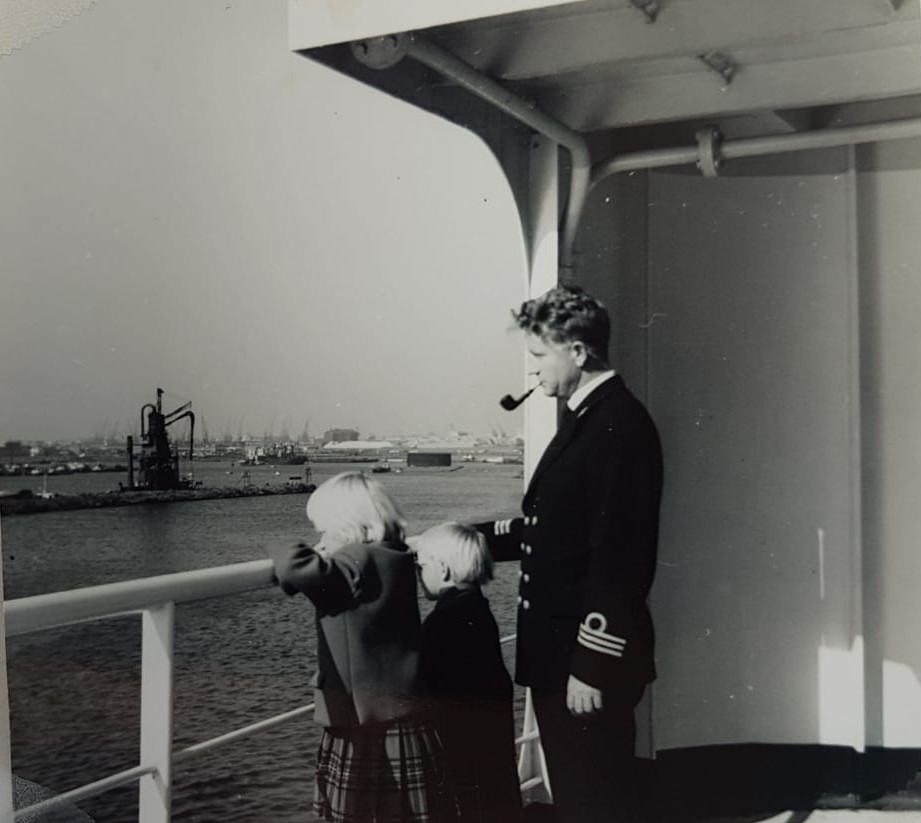
\includegraphics[width=\textwidth]{image52}
    \caption{Met de kinderen mee varen met Joop.}
\end{figure}

Ik was veel alleen met de kinderen maar ja, dat doe je gewoon en je moet niet vergeten, dat ik al langer zelfstandig was. Er waren wel vrouwen die het niet redden alleen. Dan moest de man een walbaan zoeken. Dat was het laatste wat ik Joop aan wilde doen, want hij vond het varen zo leuk. En ik kon er ook wel tegen.

\begin{figure}[h]
    \begin{centering}
    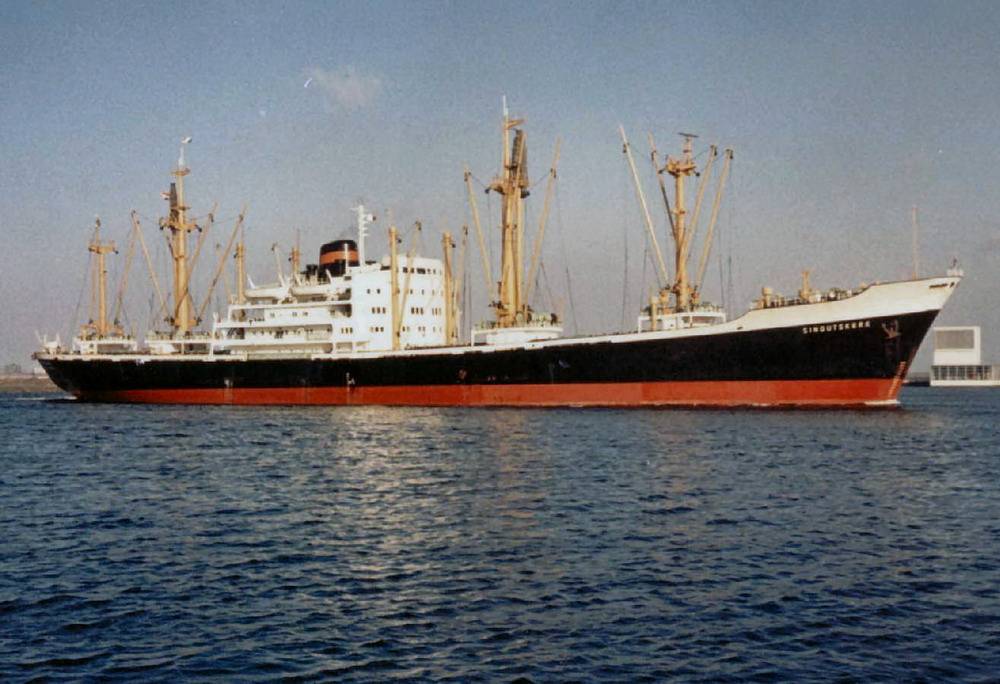
\includegraphics[width=.9\textwidth]{sinoutskerk.JPG}
    \caption{De Sinoutskerk, een schip waar Joop stuurman was.}
    \end{centering}
\end{figure}

Soms gingen we mee op kustreis. 

In de gang in Doorn hing een zwarte vaste telefoon. Joop belde dan wel eens, haast nooit. We hadden een keer afgesproken, toen waren de kinderen nog klein, dat hij een keer zou bellen. Toen was hij op reis. En wij zaten er helemaal klaar voor en dat is ook allemaal doorgegaan, maar we vonden het eigenlijk niks dat hij er niet bij was. Ik zei: ``Dat moet je maar niet meer doen''. Dan hoor je elkaar en dan voel je het gemis meer. En dat vonden jullie ook. 

We zeiden ooit tegen elkaar, hoe mooi het zou zijn als er een soort televisiefoon zou zijn, zodat je elkaar ook zou kunnen zien. Nou, dat is er wel gekomen (na een kerstviering via zoom vanwege de corona in 2020), maar een beetje te laat voor ons. Nou ja, je trouwt met iemand die vaart, dus zo is dat dan.

Op een gegeven moment liep ik in Doorn mijn vroegere vriendin Riekje tegen het lijf. Hoe ging dat? Ja, ik had al iemand zien lopen en dacht: ``Dat lijkt wel Riekje Bakker!'' Ik moet toch eens opletten. En toen fietste ik naar school om de kinderen op te halen en toen reed Riekje voor me! En ik riep: ``Ja, ik zie, het is haar!'' Ik kende haar van het Wilhelmina Gasthuis. Zij zat in de keukenafdeling en ik in de huishoudafdeling. Die keuken vond ik niks, met van die grote gamellen. Riekje was echt een lief mens. Jaren later woonden wij weer bij elkaar in de buurt in Drenthe. We zijn altijd vriendinnen gebleven. Jammer genoeg is ze nu overleden.

Jacqueline en Yvonne zijn opgegroeid in Doorn. Kleuterschool, Lagere school: Willem de Zwijgerschool en het Revius Lyceum. 

\begin{figure}[h]
    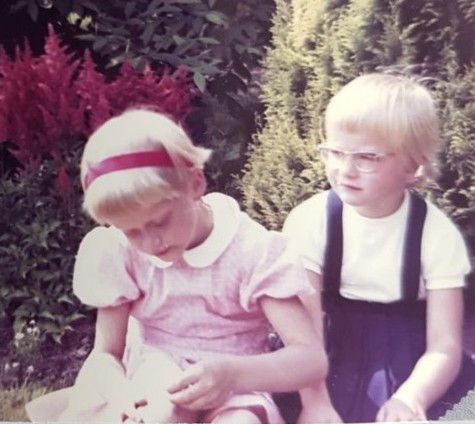
\includegraphics[width=\textwidth]{image53}
    \caption{Jacqueline en Yvonne.}
\end{figure}

In de vakanties troffen we het als Joop net met verlof was. Dan gingen we lang weg, naar Frankrijk, Spanje, Portugal of Joegoslavi\"{e}. Soms wilde ik dan wel weer naar huis.

We reden er 2 dagen over en ’s avonds dan stopten we en kampeerden we in het wild. Toen had ik net een verhaal gehoord dat mensen waren overvallen. Ik weet nog dat ik in de nacht een auto hoorde aankomen, maar het waren gewoon mensen die ook een plekje voor de nacht zochten. Die hadden ons zien staan en kwamen daar ook slapen.

\begin{figure}[h]
    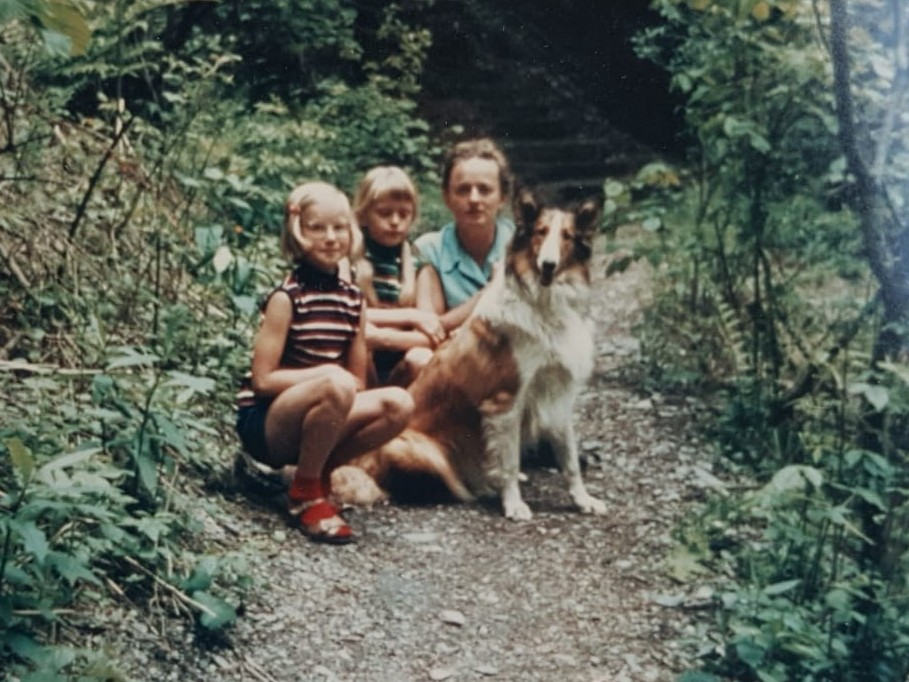
\includegraphics[width=\textwidth]{image54}
    \caption{Met de hond op de foto.}
\end{figure}

Toen de kinderen 6 en 7 waren hebben we eerst een tent gehuurd en daarna een bungalowtent gekocht. De stokken waren gemerkt. In Luxemburg gingen we kamperen met zijn drie\"{e}n toen Joop niet meekon, en zo konden we de tent ook samen opzetten.

Ik vond dat er een hond bij moest. Bij mijn ouders was ook een hond, Blacky, toen wij als kinderen nog thuis waren en bij Joop thuis ook (ook al wandelden ze er niet zo veel mee).

Timba ging altijd mee wandelen op vakantie, Luxemburg, de Ardennen. En dan was hij z\'{o} moe van al het lopen. Dan legde ik wat vlees op zijn neus en hij was z\'{o} moe dat hij nergens meer op reageerde!

\begin{figure}[h]
    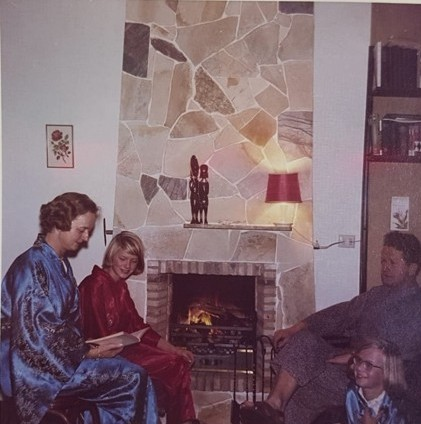
\includegraphics[width=\textwidth]{image55}
    \caption{Het gezin rond de haard.}
\end{figure}

Eerst hadden we in Doorn een schattig kacheltje wat we ook al in Dordrecht hadden, maar in Doorn was de kamer groter en kwam er een andere kachel, gestookt op kolen. Achter de garage was een kolenhok. Het was een makkelijke kachel, als hij \'{e}\'{e}n keer brandde deed hij het de hele dag. Maar het was wel ideaal toen we centrale verwarming kregen. En een open haard.

We hebben v\'{e}\'{e}l gewandeld in Doorn! Toen we eenmaal in het huis in Doorn woonden was dat eigenlijk de mooiste tijd. Het mooiste wonen ook. 

Het was een mooi plekje, zo bij het bos en een ruim huis. Het zorgen voor de vogels hoorde dar ook bij, dat deed mijn moeder ook en de buurvrouw Betty. Later werd de keuken nog verbouwd en kreeg Jacqueline een zolderkamer en Yvonne een dakterras aan haar kamer, die kleiner was met een opklapbed. Er was een barretje in de keuken en een open verbinding met de kamer. Veel gemakkelijker.

Toen de kinderen groter waren heb ik nog met ouderen gewerkt als vrijwilligster. Dat was wel leuk. Een betaalde baan was niet noodzakelijk en was druk. De jeugd is wel veranderd werd ik gewaarschuwd. Daarom heb ik nooit meer betaald werk gezocht.

In het eindexamenjaar heb ik heel wat zitten overhoren en toen gingen de kinderen tegelijk de deur uit. Jacqueline was een jaartje ouder (18) en ging studeren. Omdat Jacqueline ging, ging Yvonne ook uit huis. Zij was 17. Toen heb ik wel even moeten wennen. 

Met Joop ging het in die tijd ook niet altijd goed.